%% ----------------------------------------------------------------
%%? 1st Draft In Progress
%% ---------------------------------------------------------------- 
\chapter{Design/Method (780 words)}

\section{Non-Functional Requirements}
The software application was designed with the following guidelines in mind:\begin{itemize}
    \item \textbf{
        Synergy with existing software
    } \(\to\) the features in the application should be able to be inserted in existing music streaming applications without issue (such as Spotify, Apple Music, etc.) %! How did I ensure this?
    \item \textbf{
        Desktop only
    } \(\to\) to simplify the development process, the application was only developed for use on desktop
    \item Users can access their library in 3 clicks or less %? Arbitrary amount of clicks | is this necessary?
    \item All controls should be intuitive and comfortable to use
\end{itemize} %! What other non-functional requirements do I have?

\section{Functional Requirements}
Note: the below list of functional requirements have their MoSCoW prioritisations in bold.
\begin{itemize}
    % Spotify OAuth authorisation flow
    \item[\textbf{Auth1}] Users \textbf{must} be able to access their library by logging in with the credentials of the platform that library is stored in.
    \item[\textbf{Auth2}] The system \textbf{must} be able to interact with a user's library by using a user-specific API access token.
    % Get all songs + all playlists from user's library
    \item[\textbf{Lib1}] Users \textbf{must} be able to view all songs from a singular playlist
    \item[\textbf{Lib2}] Users \textbf{should} be able to view view multiple/all playlists in their collection at once
    % Getting the Echo Nest Attributes
    \item[\textbf{Attr}] Each song in the user's library \textbf{must} have the appropriate Echo Nest attributes attached
    % Playback Control
    \item[\textbf{Play}] Users \textbf{should} be able to control playback on another device that is playing their music
    % Table View
    \item[\textbf{Table}] Users \textbf{must} be able to see the metadata and attributes for all their songs in a table
    % Static Graph 1D, 2D, 3D
    \item[\textbf{SG1}] Users \textbf{should} be able to see their songs mapped along one dimension for each attribute
    \item[\textbf{SG2}] Users \textbf{must} be able to see their songs mapped along 2 dimensions for each combination of 2 continuous attributes
    \item[\textbf{SG3}] Users \textbf{must} be able to see their songs mapped along 3 dimensions for each combination of 3 continuous attributes
    % Detailed Song View + Neighbours
    \item[\textbf{DeSo1}] Users \textbf{must} be able to see the attributes and metadata for a song when they click on it.
    \item[\textbf{DeSo2}] Users \textbf{should} be able to see the most similar songs to the currently selected song
    % Dynamic Graph
    \item[\textbf{DG1}] The system \textbf{must} create a logical similarity graph of all the songs currently being viewed
    \item[\textbf{DG2}] The system \textbf{must} be able to render logical dynamic graph in 2D
    \item[\textbf{DG3}] The system \textbf{must} be able to render logical dynamic graph in 3D
    \item[\textbf{DG4}] Users \textbf{must} be able to toggle which attributes and metadata are currently affecting the similarity graph
    % Filtering
    \item[\textbf{Fil1}] Users \textbf{should} be able to filter songs on any view using continuous attributes/metadata
    \item[\textbf{Fil2}] Users \textbf{should} be able to filter songs on any view using discrete attributes/metadata
    \item[\textbf{Fil3}] Users \textbf{should} be able to toggle which playlists are currently being shown
    % Visualising Listening Journeys
    \item[\textbf{VLJ1}] Users \textbf{must} be able to see their currently playing song as a distinct node in the graph views.
    \item[\textbf{VLJ2}] Users \textbf{must} be able to see their queue as a directed line through the relevant songs
    \item[\textbf{VLJ3}] Users \textbf{should} be able to see their history rendered as a fading line (up to different preset lengths(of either number of songs or length of time))
    % Controlling Listening Journeys
    \item[\textbf{CLJ1}] Users \textbf{should} be able to set a target song for the listening journey to go to
    \item[\textbf{CLJ2}] Users \textbf{must} be able to select a song to randomly listen around
    \item[\textbf{CLJ3}] Users \textbf{must} be able to create a segment of the listening journey where the songs are played through in a fixed order
    \item[\textbf{CLJ4}] Users \textbf{must} be able to create a segment of the listening journey where songs are played through randomly
    \item[\textbf{CLJ5}] Users \textbf{should} be able to listen to a song and then return to their original listening journey trajectory (effectively a temporary diversion)
    % Past and Present Listening Journeys
    \item[\textbf{PLJ1}] Users \textbf{should} be able to view past audio journeys (segments of their full audio history), possibly as a sped up line
    \item[\textbf{PLJ2}] Users \textbf{should} be able to quickly re-listen to an old audio journey
    % User-added song tags
    \item[\textbf{Tag1}] Users \textbf{should} be able to add custom tags to their songs (these can then be used to make the song similarity more informative)
    \item[\textbf{Tag2}] The system \textbf{should} treat these tags in a similar fashion to genres, in that they are hierarchical and not mutually exclusive
\end{itemize}

\begin{figure}
    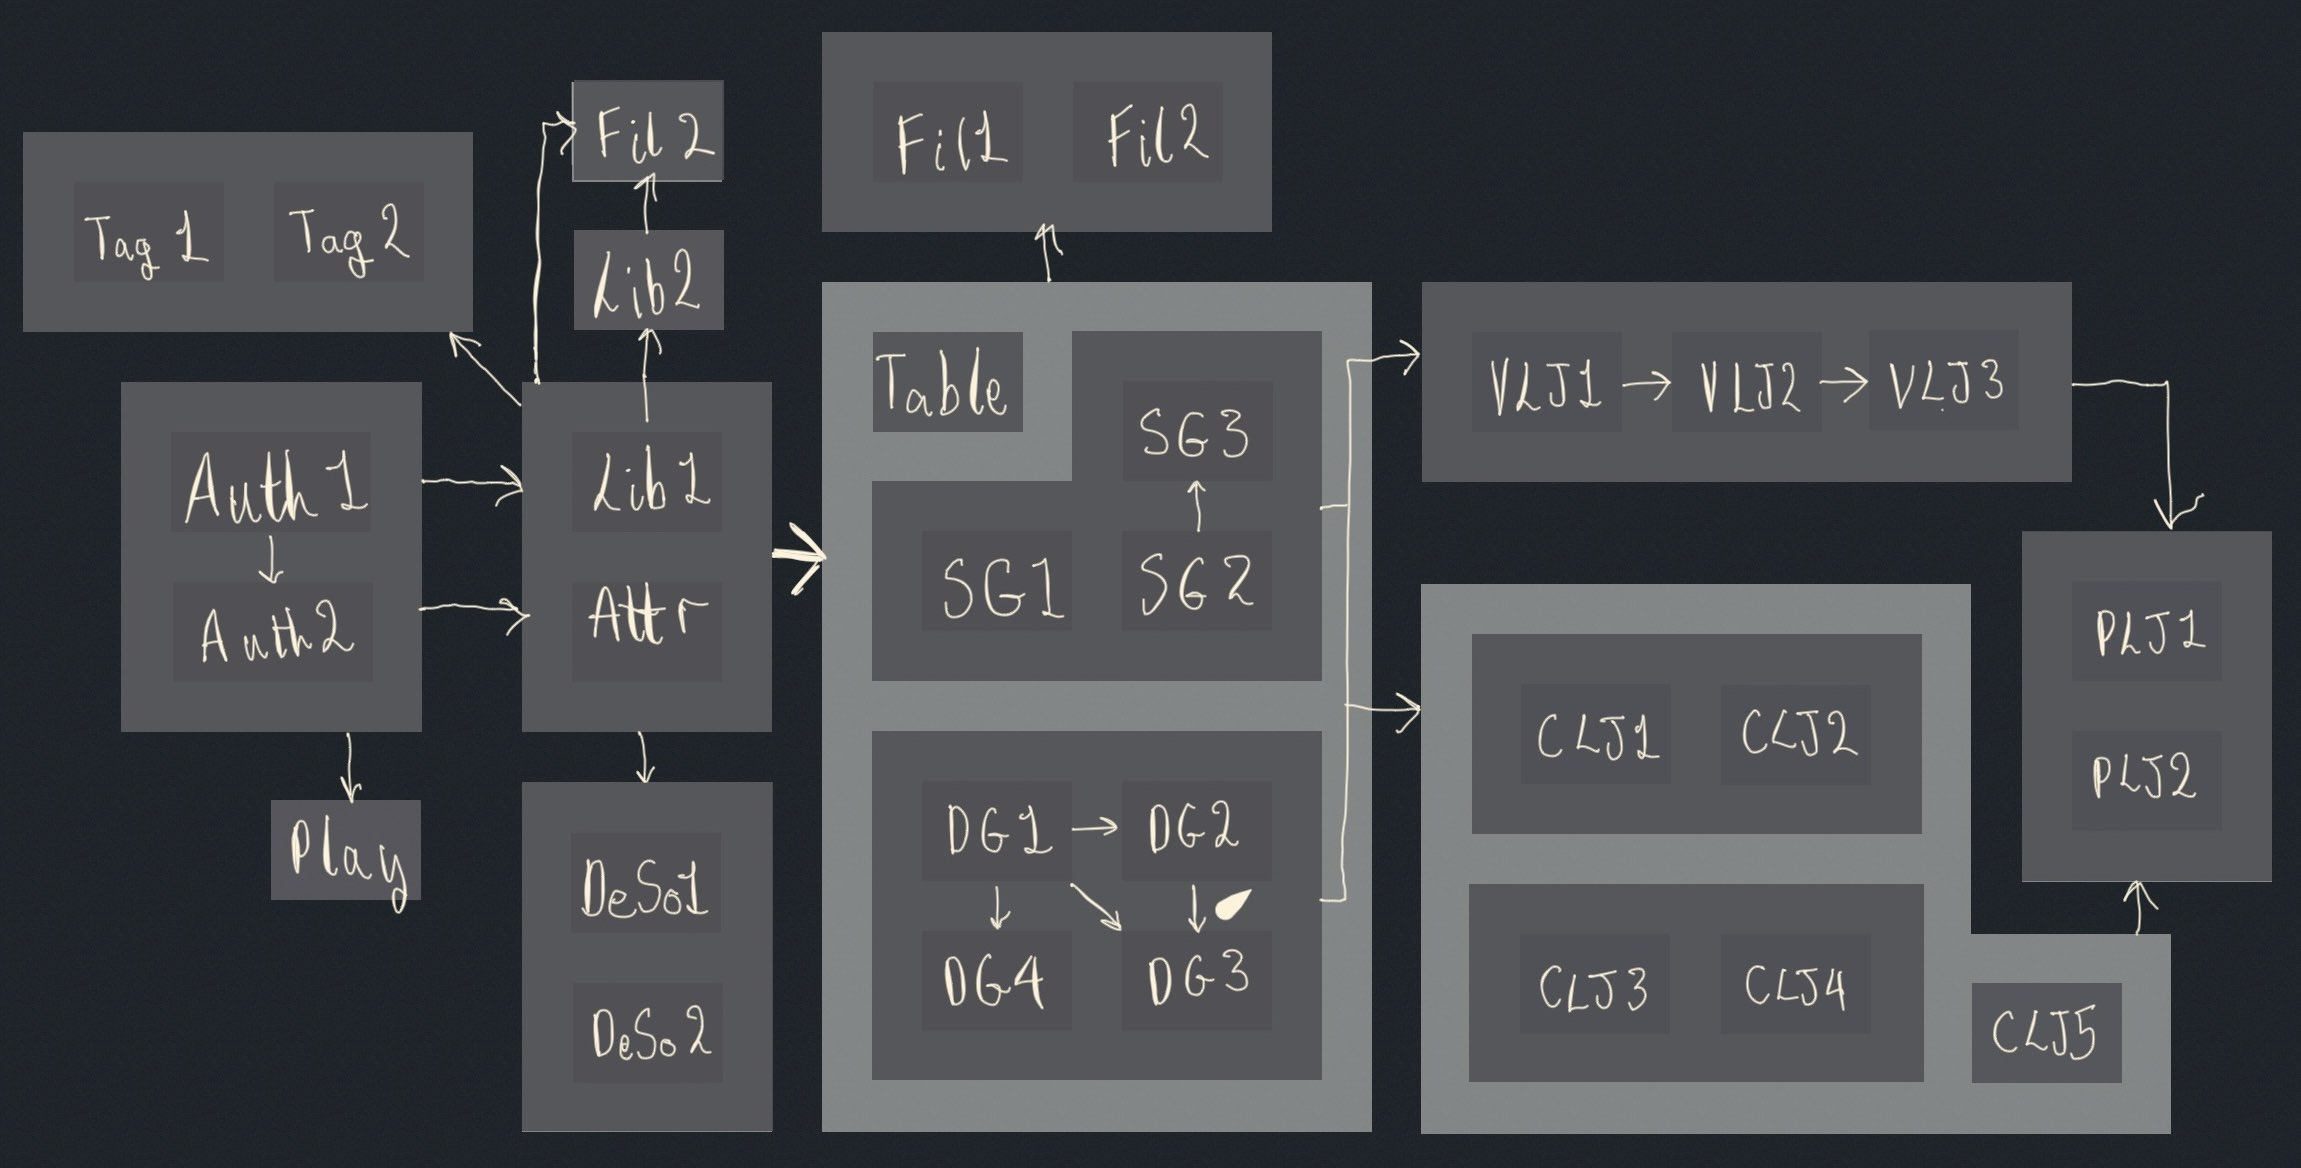
\includegraphics[scale=0.204]{Activity_Network_Diagram.jpg}
    \caption{Activity Network Diagram of Functional Dependencies}
\end{figure}

% User stories have been cut as it was deemed that their content overlapped too much with the functional requirements and as such were easy to cut to fit within the word limit

\section{TODO: Static Cartesian Graphs}
%* Explain how I coded this basically
[-] combine the different continuous attributes
[-] 

\section{Dynamic Similarity Graph}
[-] Each song is a node in the graph
[-] Each song has multiple bidirectional weighted edges to each other song
    [-] Discrete attributes/metadata: edge is overlap of discrete metric between song A and song B
    [-] Continuous attributes/metadata: weight of edge is the 1-x, where x is a the difference between the values of Song A's acousticness and Song B's acousticness (for example)
[-] When rendering the graph, songs are pulled closer together depending on strength of weight:
    [-] continuous weight of 100\% - songs pulled as close together as possible
[?] maybe have a toggle to turn off collisions? that way clusters that form might be more interesting or the graph never settles on a shape

\section{Audio Journeys}

\section{TODO: UI Wireframes}%* can categorise them by the feature roadmap? Or maybe I can group sections of the roadmap
As one of the key non-functional requirements is for the developed features to integrate into existing streaming applications, the UI was designed using Spotify's desktop interface as an inspiration.

\section{TODO: Storyboards}%? How many do I have of these?

%todo how do I fit this into the project. Is it design or development
%TC: ignore
\begin{longtable}[c]{|c|c|c|p{5em}|p{5.5em}|}
    \caption{The Echo Nest Attributes}\\%todo better caption
    \toprule
    \textbf{Attribute} & \textbf{Definition} & \textbf{Datatype} & \textbf{Possible Values} & \textbf{Continuous /Discrete} \\
    \midrule
    \endfirsthead

    \textbf{Acousticness} & & \texttt{float} & \texttt{0}-\texttt{1} & \multirow{9}{*}{Continuous}\\*
    \cmidrule{1-4}
    \textbf{Danceability} & & \texttt{float} & \texttt{0}-\texttt{1} & \\*\cmidrule{1-4}
    \textbf{Energy} & & \texttt{float} & \texttt{0}-\texttt{1} & \\*\cmidrule{1-4}
    \textbf{Instrumentalness} & & \texttt{float} & \texttt{0}-\texttt{1} & \\*\cmidrule{1-4}
    \textbf{Liveness} & & \texttt{float} & \texttt{0}-\texttt{1} & \\*\cmidrule{1-4}
    \textbf{Loudness} & & \texttt{float} & \texttt{-60}-\texttt{0} & \\*\cmidrule{1-4}
    \textbf{Speechiness} & & \texttt{float} & \texttt{0}-\texttt{1} & 
    \\*\cmidrule{1-4}
    \textbf{Valence} & & \texttt{float} & \texttt{0}-\texttt{1} & \\*\cmidrule{1-4}
    \textbf{Tempo} & & \texttt{float} & \(\ge\)\texttt{0} & \\*
    \midrule
    \textbf{Key} & & \texttt{integer} & \texttt{None}/\texttt{C}/\texttt{C\#} /\texttt{D}/\texttt{D\#}/\texttt{E}/\texttt{F} /\texttt{F\#}/\texttt{G}/\texttt{G\#}/ \texttt{A}/\texttt{A\#}/\texttt{B} & \multirow{3}{*}{Discrete}\\*
    \cmidrule{1-4}
    \textbf{Mode} & & \texttt{boolean} & \texttt{true}/\texttt{false} & \\*
    \cmidrule{1-4}
    \textbf{Time Signature} & & \texttt{integer} & \texttt{3}/\texttt{4}/\texttt{5}/\texttt{6}/\texttt{7} & \\*
    \midrule
    
\end{longtable}
%TC: endignore